\documentclass[12pt, %larger font size
			  t     %frames are top-aligned
]{beamer}%
\mode<presentation>

\usetheme{Garching}

\usepackage[utf8]{inputenc}
\usepackage[english,ngerman]{babel}%
\usepackage[autostyle=true]{csquotes}%
\usepackage{graphicx}
\usepackage[export]{adjustbox} % to align images
\usepackage{booktabs}
\usepackage{multimedia} % for /media to embed videos

\title{Post-Processing of Manipulation Trajectories}%
\subtitle{Internship Report}%
\author[Excellent]{Sarah Braun}%
\institute[TU München]{Technische Universität München}%
\titlegraphic{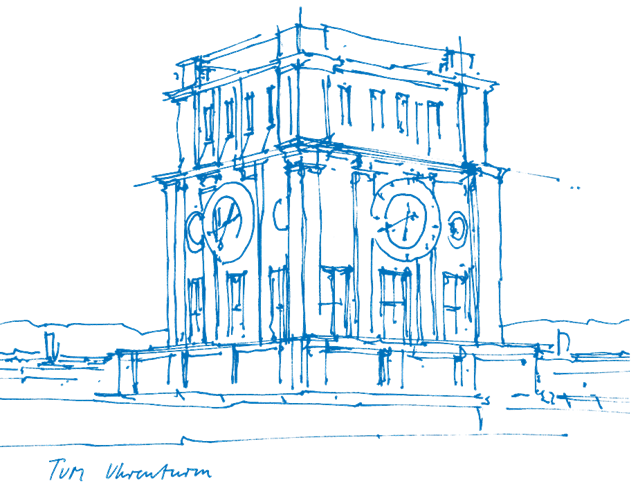
\includegraphics[height=0.3\paperheight]{tum-uhrenturm}}
\date{July 24th, 2017}%


\begin{document}
\selectlanguage{english}

%-------TITLEFRAME-----------------------------------------------------------------------
\begin{frame}[plain]
  \titlepage
\end{frame}

%-------POST-PROCESSING STRATEGIES-------------------------------------------------------
\begin{frame}
  \frametitle{Evaluation of Various Post-Processing Strategies}
  \begin{enumerate}
  \item Hauser's shortcutting idea
  \item Smooth object interaction
  \item Sampling of new transitions
  \item \textcolor{gray}{Sampling of new grasps and placements}
  \end{enumerate}
\end{frame}

%-------HAUSER SHORTCUTTING-------------------------------------------------------------
\begin{frame}
 \frametitle{Hauser's Shortcutting Idea}

 \begin{columns}[T]
   \begin{column}{.5\textwidth}
     \begin{itemize}
     \item \only<1>{sample two points} \only<2->{\textcolor{gray}{sample two points}}
     \item\only<1>{compute shortcut}\only<2->{compute shortcut \textcolor{orange}{How?}}
     \item \only<1>{check collisions} \only<2->{\textcolor{gray}{check collisions}}
     \end{itemize}
   \end{column}
   
   \begin{column}{.5\textwidth}
     \includegraphics[height=0.6\paperheight, right]{../Hauser_Shortcutting.pdf}
   \end{column}
 \end{columns}
\end{frame}

%-------SYNCHRONIZATION OF AXES-------------------------------------------------------------
\begin{frame}
\frametitle{Synchronization of Axes}
\vskip -.3cm
\begin{columns}[T]
  \begin{column}{.5\textwidth}
    \begin{block}{Basic Idea}
      \begin{itemize}
        \item find "bottleneck" axis
	    \item synchronize all axes to bottleneck time
	  \end{itemize}
	\end{block}
  \end{column}

  \only<-2>{
  \begin{column}{.5\textwidth}
    \invisible{
    \begin{block}{Reflexxes}
      \begin{itemize}
        \item find "bottleneck axis" and inoperative time intervals
        \item synchronize all axes to earliest possible point in time
      \end{itemize}
    \end{block}}
  \end{column}
  }

  \only<3>{
  \begin{column}{.5\textwidth}
    \begin{block}{Reflexxes}
      \begin{itemize}
        \item find "bottleneck axis" and inoperative time intervals
        \item synchronize all axes to earliest possible point in time
      \end{itemize}
    \end{block}
  \end{column}
  }
\end{columns}

\vskip -1cm
\hskip -.57cm
\only<2>{
\textbf{\textcolor{orange}{Problem}}
\setlength{\leftmargini}{.4cm}
\begin{itemize}
  \item  synchronization to arbitrary subsequent point in time not always possible
  \item each axis has inoperative time intervals in which axis cannot be synchronized
  \end{itemize}
}

\end{frame}

%-------SMOOTH INTERACTION-------------------------------------------------------------
\begin{frame}
\frametitle{Smooth Interaction}
  \begin{itemize}
    \item "interaction" = approaching the object to be gripped
  \end{itemize}

  \only<1>{
  \centering
    \fbox{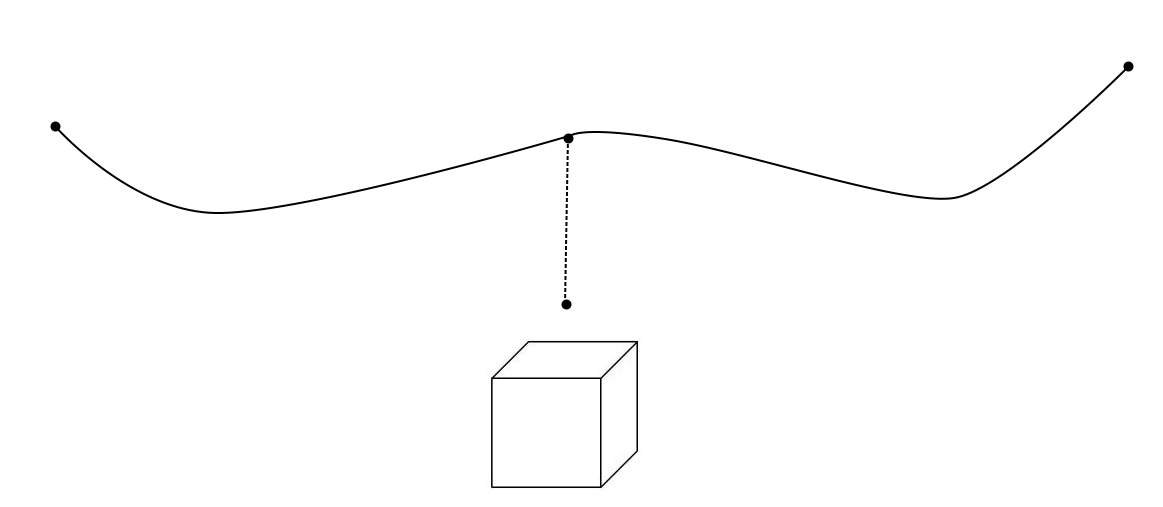
\includegraphics[scale=0.2]{../SmoothInteraction_smaller.jpg}}
    \begin{itemize}
      \item stopping takes a lot of time\\
      \invisible{test}
    \end{itemize}
  }  
  \only<2>{
    \centering
    \fbox{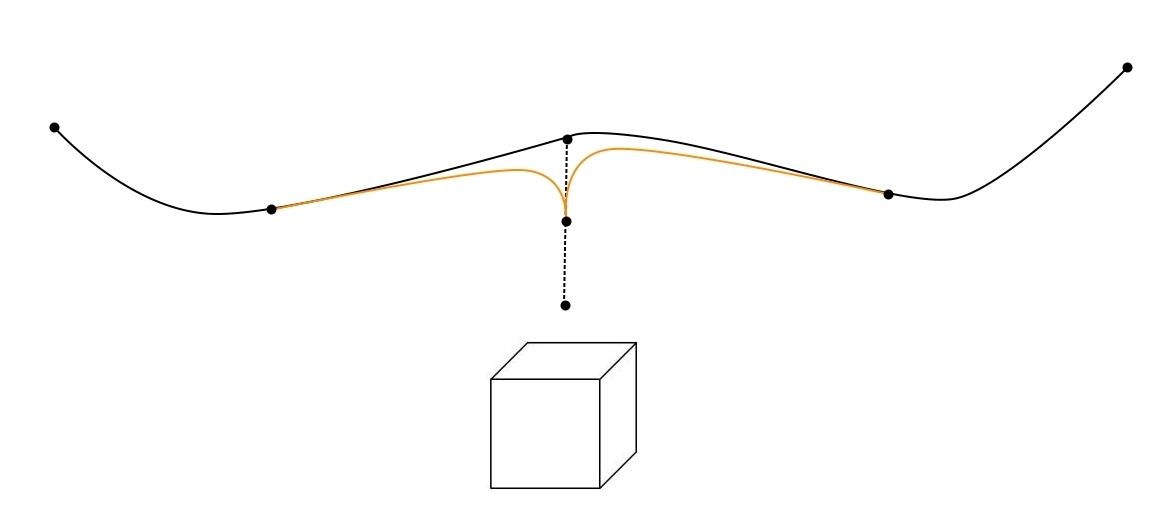
\includegraphics[scale=0.2]{../SmoothInteraction_smaller_orange.jpg}}
    \begin{itemize}
      \item better: slide smoothly into linear movement
      \item use Reflexxes for computation of orange motion
    \end{itemize}
  }
  
  
\end{frame}

%-------TRANSITION SAMPLING---BASIC IDEA-----------------------------------------------
\begin{frame}
\frametitle{Sampling of New Transitions - Basic Idea}
\begin{itemize}
  \item Recall: Manipulation Planner\\ 
        \textcolor{red}{PHILIPP'S IMAGE}
  \item Idea: Sample new transitions and re-plan trajectories in adjacent modes
\end{itemize}


\end{frame}

%-------TRANSITION SAMPLING---MORE DETAILS-----------------------------------------------
\begin{frame}
\frametitle{Sampling of New Transitions - More Details}
\begin{itemize}
  \item new transition is ... 
  \begin{itemize}
    \item ... either new inverse kinematic \textcolor{red}{include picture}
    % picture: object with schematic  robot, arrow, object at same position, same grasp, same robot base but different joint positions
    % Im_1
    \item ... or arbitrary valid configuration \textcolor{red}{include picture}
    % picture: schematic robot in two different configurations
    % Im_2
  \end{itemize}
  \item Replan using Reflexxes:\\ \textcolor{red}{include picture similar to Philipp's}
  % two manifolds, transition area, new transition in different color, sampled point and Reflexxes' connection also in different color
  % Im_3
  
\end{itemize}


\end{frame}

%-------GRASP SAMPLING--------------------------------------------------------------
\begin{frame}
\frametitle{Sampling of New Grasps and Placements}
\begin{itemize}
  \item Recall: Within-contact roadmaps for a couple of \textit{fixed} grasps and placements
  \item Idea: Also sample new grasps and replan
  \item Difficulties: new grasp changes planning scene for all subsequent modes, expensive updates
  \item \textcolor{red}{Evtl auch hier Grafik}
  % Bild von Philipp mit roadmap of roadmaps, streiche hier eine roadmap durch und ersetze sie durch eine neue, zu neuem Grasp gehörend
\end{itemize}


\end{frame}

%-------EVALUATION---BEFORE PP-----------------------------------------------------
\begin{frame}
\frametitle{Evaluation}
\vskip -.3cm
Simple pick-and-place task \textcolor{orange}{without} Post-Processing
\only<1>{ % VELOCITY DIAGRAM
\begin{center}
  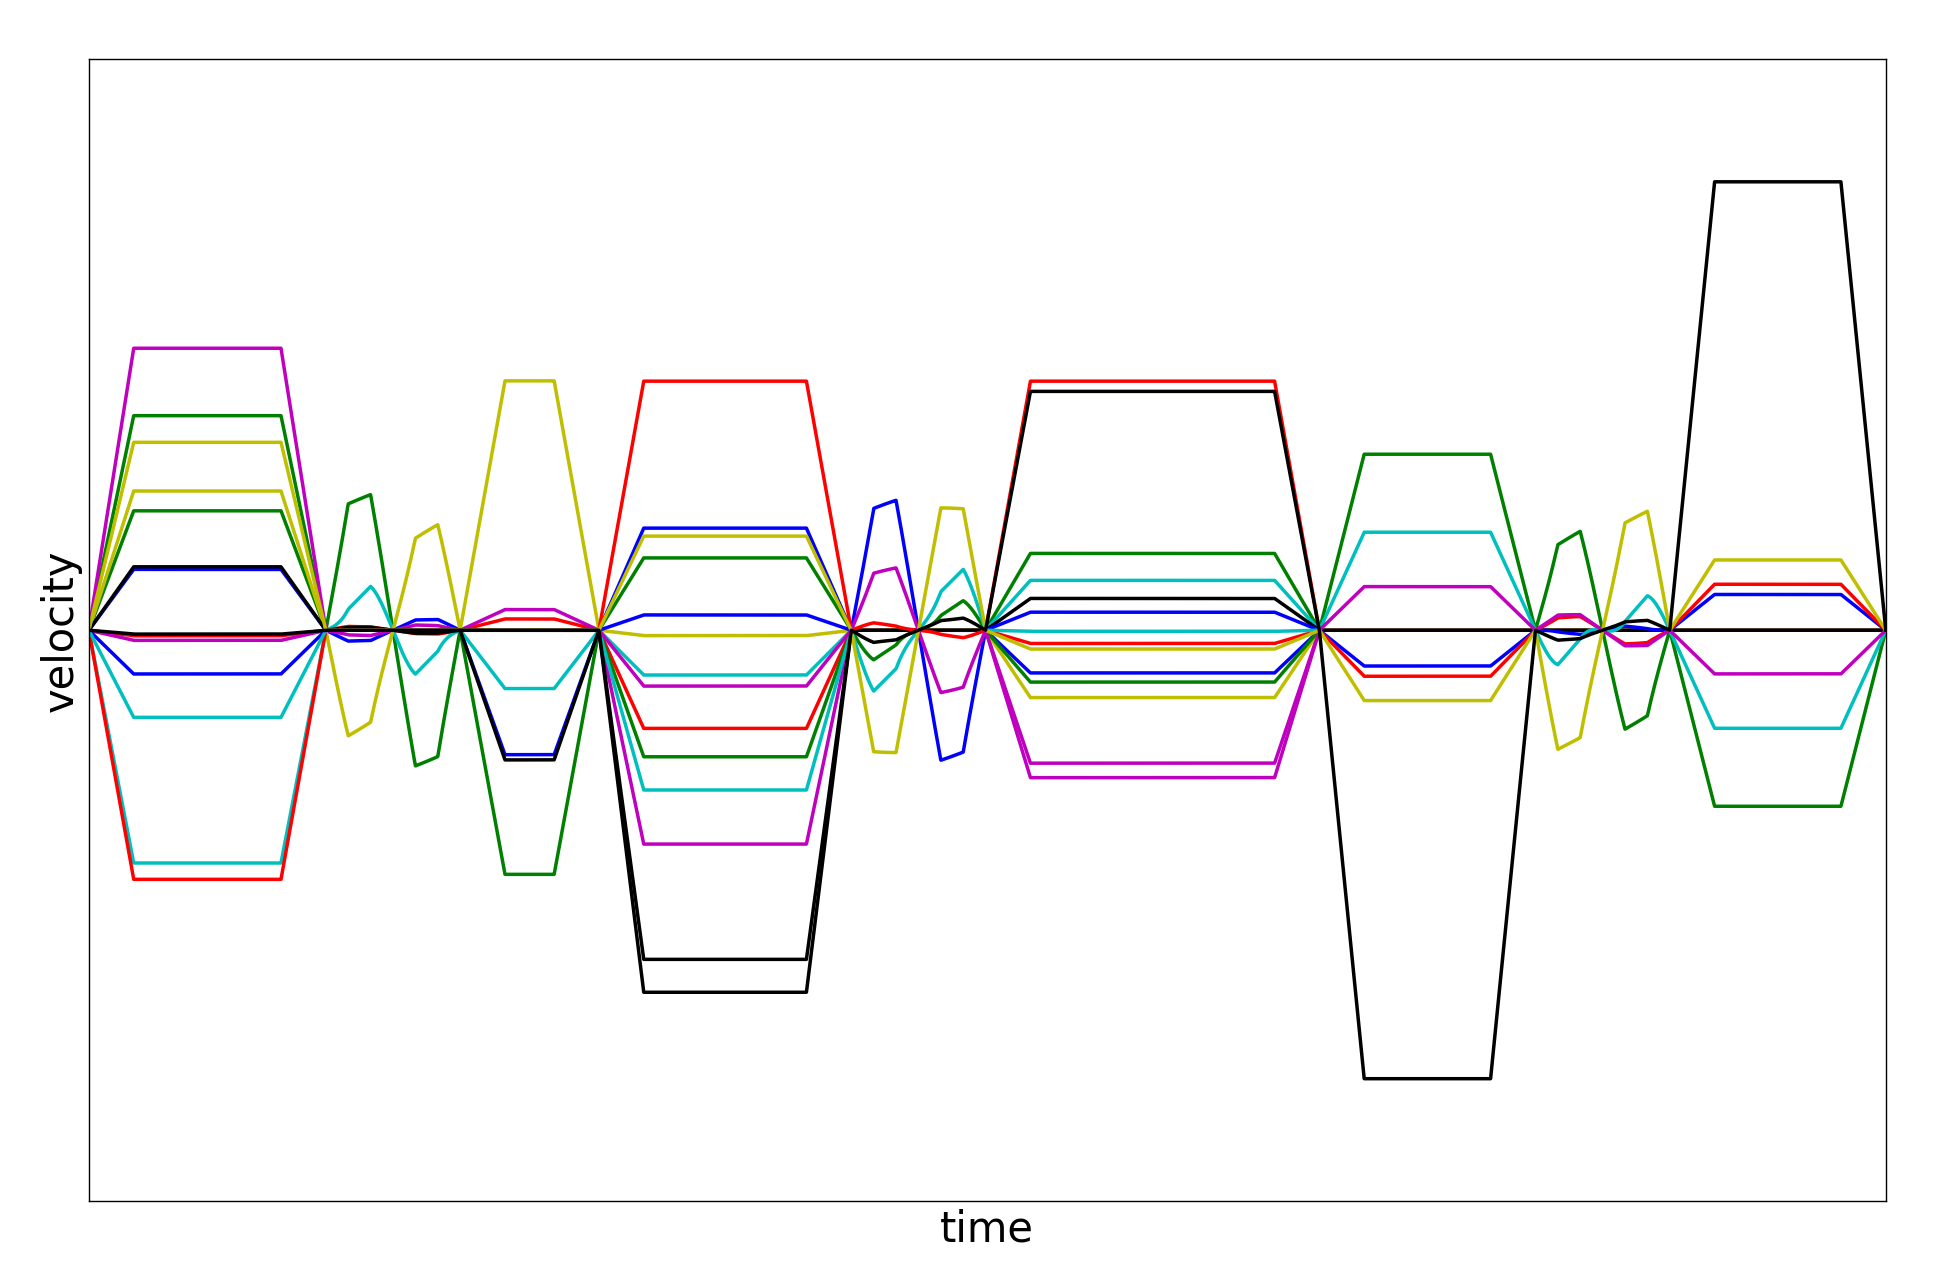
\includegraphics[scale=0.13]{../Record_8/Step1.png}
\end{center}
}

\only<2>{ % VIDEO
  \centering
  \movie[height = 6cm, width = 5.4cm, showcontrols, poster]{}{../Record_8/Step1_1.mkv}
}
\end{frame}


%-------EVALUATION---AFTER PP-----------------------------------------------------
\begin{frame}
\frametitle{Evaluation}
\vskip -.3cm
Simple pick-and-place task \textcolor{orange}{after} Post-Processing
\only<1>{ % VELOCITY DIAGRAM
\begin{center}
  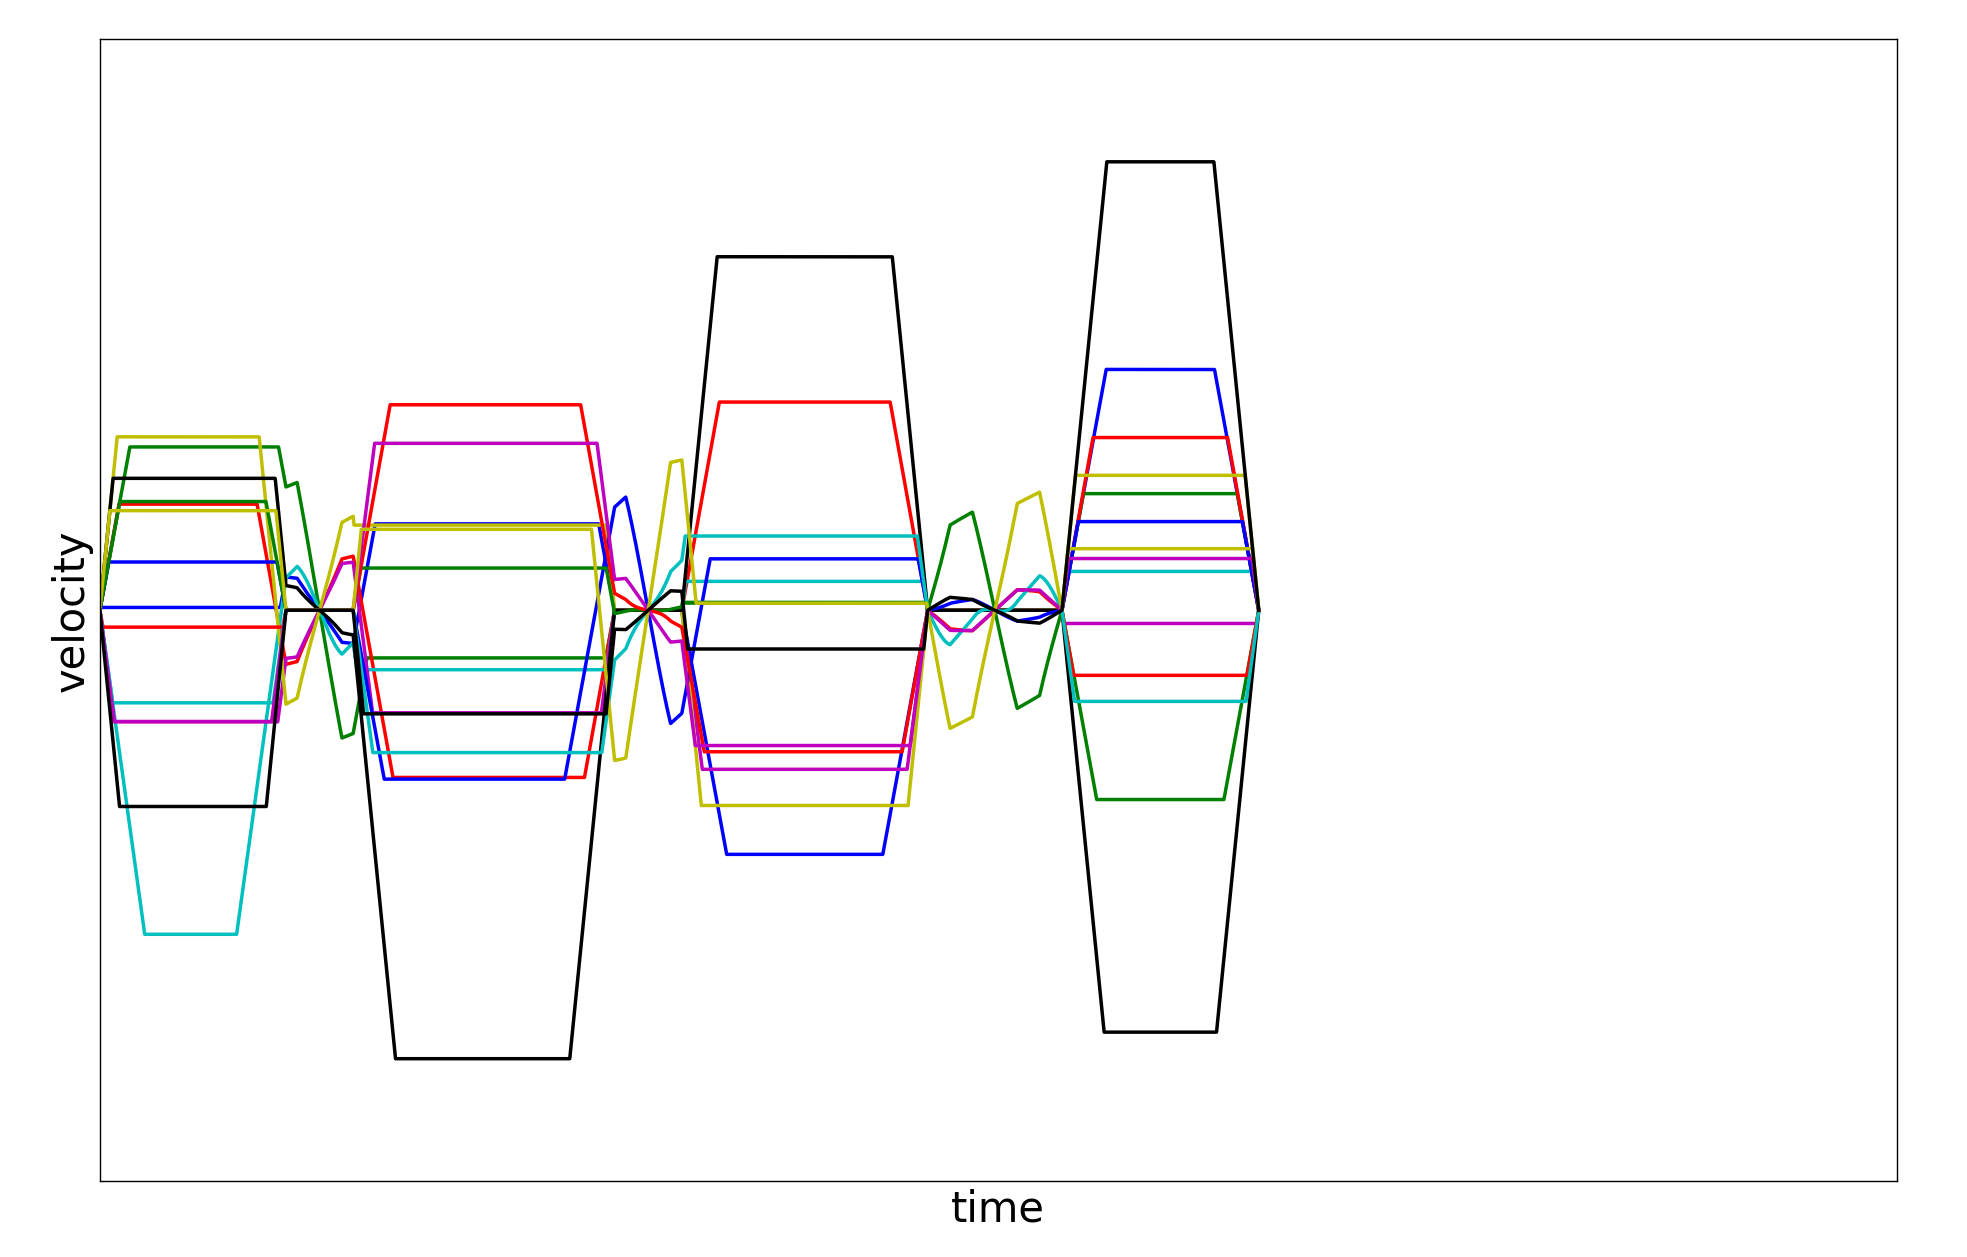
\includegraphics[scale=0.13]{../Record_8/Step4.png}
\end{center}
}

\only<2>{ % VIDEO
  \centering
  \movie[height = 6cm, width = 5.4cm, showcontrols, poster]{}{../Record_8/Step4_2.mkv}
}
\end{frame}

%-------COMPARISON-----------------------------------------------------
\begin{frame}
\frametitle{Comparison of the Post-Processing Steps}
%\includegraphics[scale=0.5]{}
\end{frame}
\end{document}
